\chapter{\emph{Measuring the State of the Art}: Understanding Commercial 360\degree{} Live Video Streaming Services} \label{chap:360video}



\section{Introduction}
Personalized 360\degree{} live video streaming is an increasingly popular mobile service that allows a broadcaster to share panoramic videos in real time with worldwide viewers. Compared to video-on-demand (VOD) streaming, experimenting with live broadcast is harder due to its intrinsic live nature, the need for worldwide viewers, and a more complex data collection pipeline. In addition, 360\degree{} live video requires much higher bandwidth to provide the same perceived quality as regular
video streaming. It has more
stringent Quality of Experience (QoE) requirements to prevent VR
motion sickness, and it incurs higher workload across all entities:
\emph{broadcasters}, \emph{streaming infrastructure}, and \emph{viewers}.


We provide insights from today’s commercial live video streaming services. The overall goals are two-fold. First, due to
a lack of measurement tools, we develop a measurement system
called LIME (LIve video MEasurement platform), which allows researchers
to conduct crowd-sourced measurements on commercial
or experimental live streaming platforms. Second, we present, to
the best of our knowledge, a first study of 360\degree{} personalized live
video streaming on commercial platforms. We select YouTube and
Facebook as the target platforms given their popularity.

We begin with developing LIME, a measurement system for live
video streaming. LIME automates the operations of one or multiple
broadcasters so that they can stream pre-recorded videos --
which enables repeatable experiments -- via both commercial (Facebook,
YouTube, Periscope, etc.) and experimental live streaming services.
LIME allows recruiting crowd-sourced viewers via Amazon
Mechanical Turk (AMT)~\cite{amt}, today’s most popular crowd-sourcing
platform. The crowd-sourced viewers are instructed to install a
Chrome extension and watch live video feeds through the platform
under test. The extension collects key performance statistics
while the viewers watch the live videos streamed from broadcasters
under LIME’s control. Note that LIME itself is a generic measurement
system that can work with both 360\degree{} and non-360\degree{} live video
broadcasting on a wide range of streaming platforms.

We leverage LIME to collect crowd-sourced measurement data
from commercial live 360\degree{} video streaming services. Specifically,
we deploy LIME and use AMT to recruit 548 viewers from 35 countries.
Our crowd-sourced viewers watched more than 4,000 minutes
of 360\degree{} live videos on YouTube and Facebook, providing a unique
\emph{viewer-side} dataset. We then conduct a comprehensive measurement
study using this dataset. We make several key observations regarding
live 360\degree{} video streaming on today’s commercial platforms. (1) Overall, the quality is not high, with 34\% (35\%) of YouTube
(Facebook) sessions having an average panoramic quality no higher
than 720p. Because only around 15\% of a panoramic scene is typically
viewed, this translates to a much lower user-perceived quality
comprised between 240p and 360p. (2) Both streaming platforms
are afflicted by long stalls, with 47\% (52\%) of YouTube (Facebook)
sessions stalling for at least 5 seconds per minute. Surprisingly, we
find such stalls are usually not attributed to the network; instead
they are likely caused by the client-side computation/rendering
overhead. (3) We develop a novel methodology for measuring the
broadcaster-to-viewer (B2V) latency, whichwe find to be non-trivial
for both YouTube (median 37.1 seconds) and Facebook (median 18.7
seconds); low-throughput sessions may have B2V latency of up to
5 minutes.

Motivated by our findings, we further leverage
LIME to conduct controlled experiments to measure how \emph{adaptiveness} 
could benefit the viewers and
the broadcaster. On the viewer side, we consider performing
viewport-adaptive streaming where the server only streams content
in the (predicted) viewport of a viewer. We find that performing
viewport-adaptive streaming effectively reduces the video encoding
bitrate by 75\% to 80\%. However, surprisingly, doing so does not
necessarily improve the video quality on Facebook and YouTube
due to several practical issues such as cautious rate adaptation design
and a limited number of quality levels. On the broadcaster
side, we use live videos and real-world cellular uplink traces to
demonstrate the potential of adaptive upload, a unique optimization
for personalized live 360\degree video streaming where the broadcaster
adaptively shrinks the view being uploaded from a full panorama
to smaller regions when the uplink bandwidth is insufficient. This
approach has potentials of significantly reducing the stall duration
(up to 99.9\% reduction in our experimented scenario) and the B2V
latency (up to 38\% reduction).

To summarize, we make the following contributions:
\begin{itemize}
	\item \textbf{The LIME System}. We develop LIME, a generic, holistic,
	and crowd-sourced measurement system for live videos.
	LIME can be used in conjunction with the majority of today’s
	commercial live video streaming platforms.
	\item \textbf{Crowd-sourced Measurement}. Leveraging LIME,
	we collect data from 548 users in 35 countries, and use this
	dataset to examine 360\degree{} live video streaming performance in
	the wild.
	\item \textbf{Controlled Experiments}. We quantify the impact of
	viewport adaptiveness on 360\degree{} live video streaming. We identify
	inefficiencies of commercial platforms that diminish the
	benefits of viewport adaptiveness.
\end{itemize}



\section{LIME Overview}

\begin{figure*}
	\footnotesize
	\begin{center}
		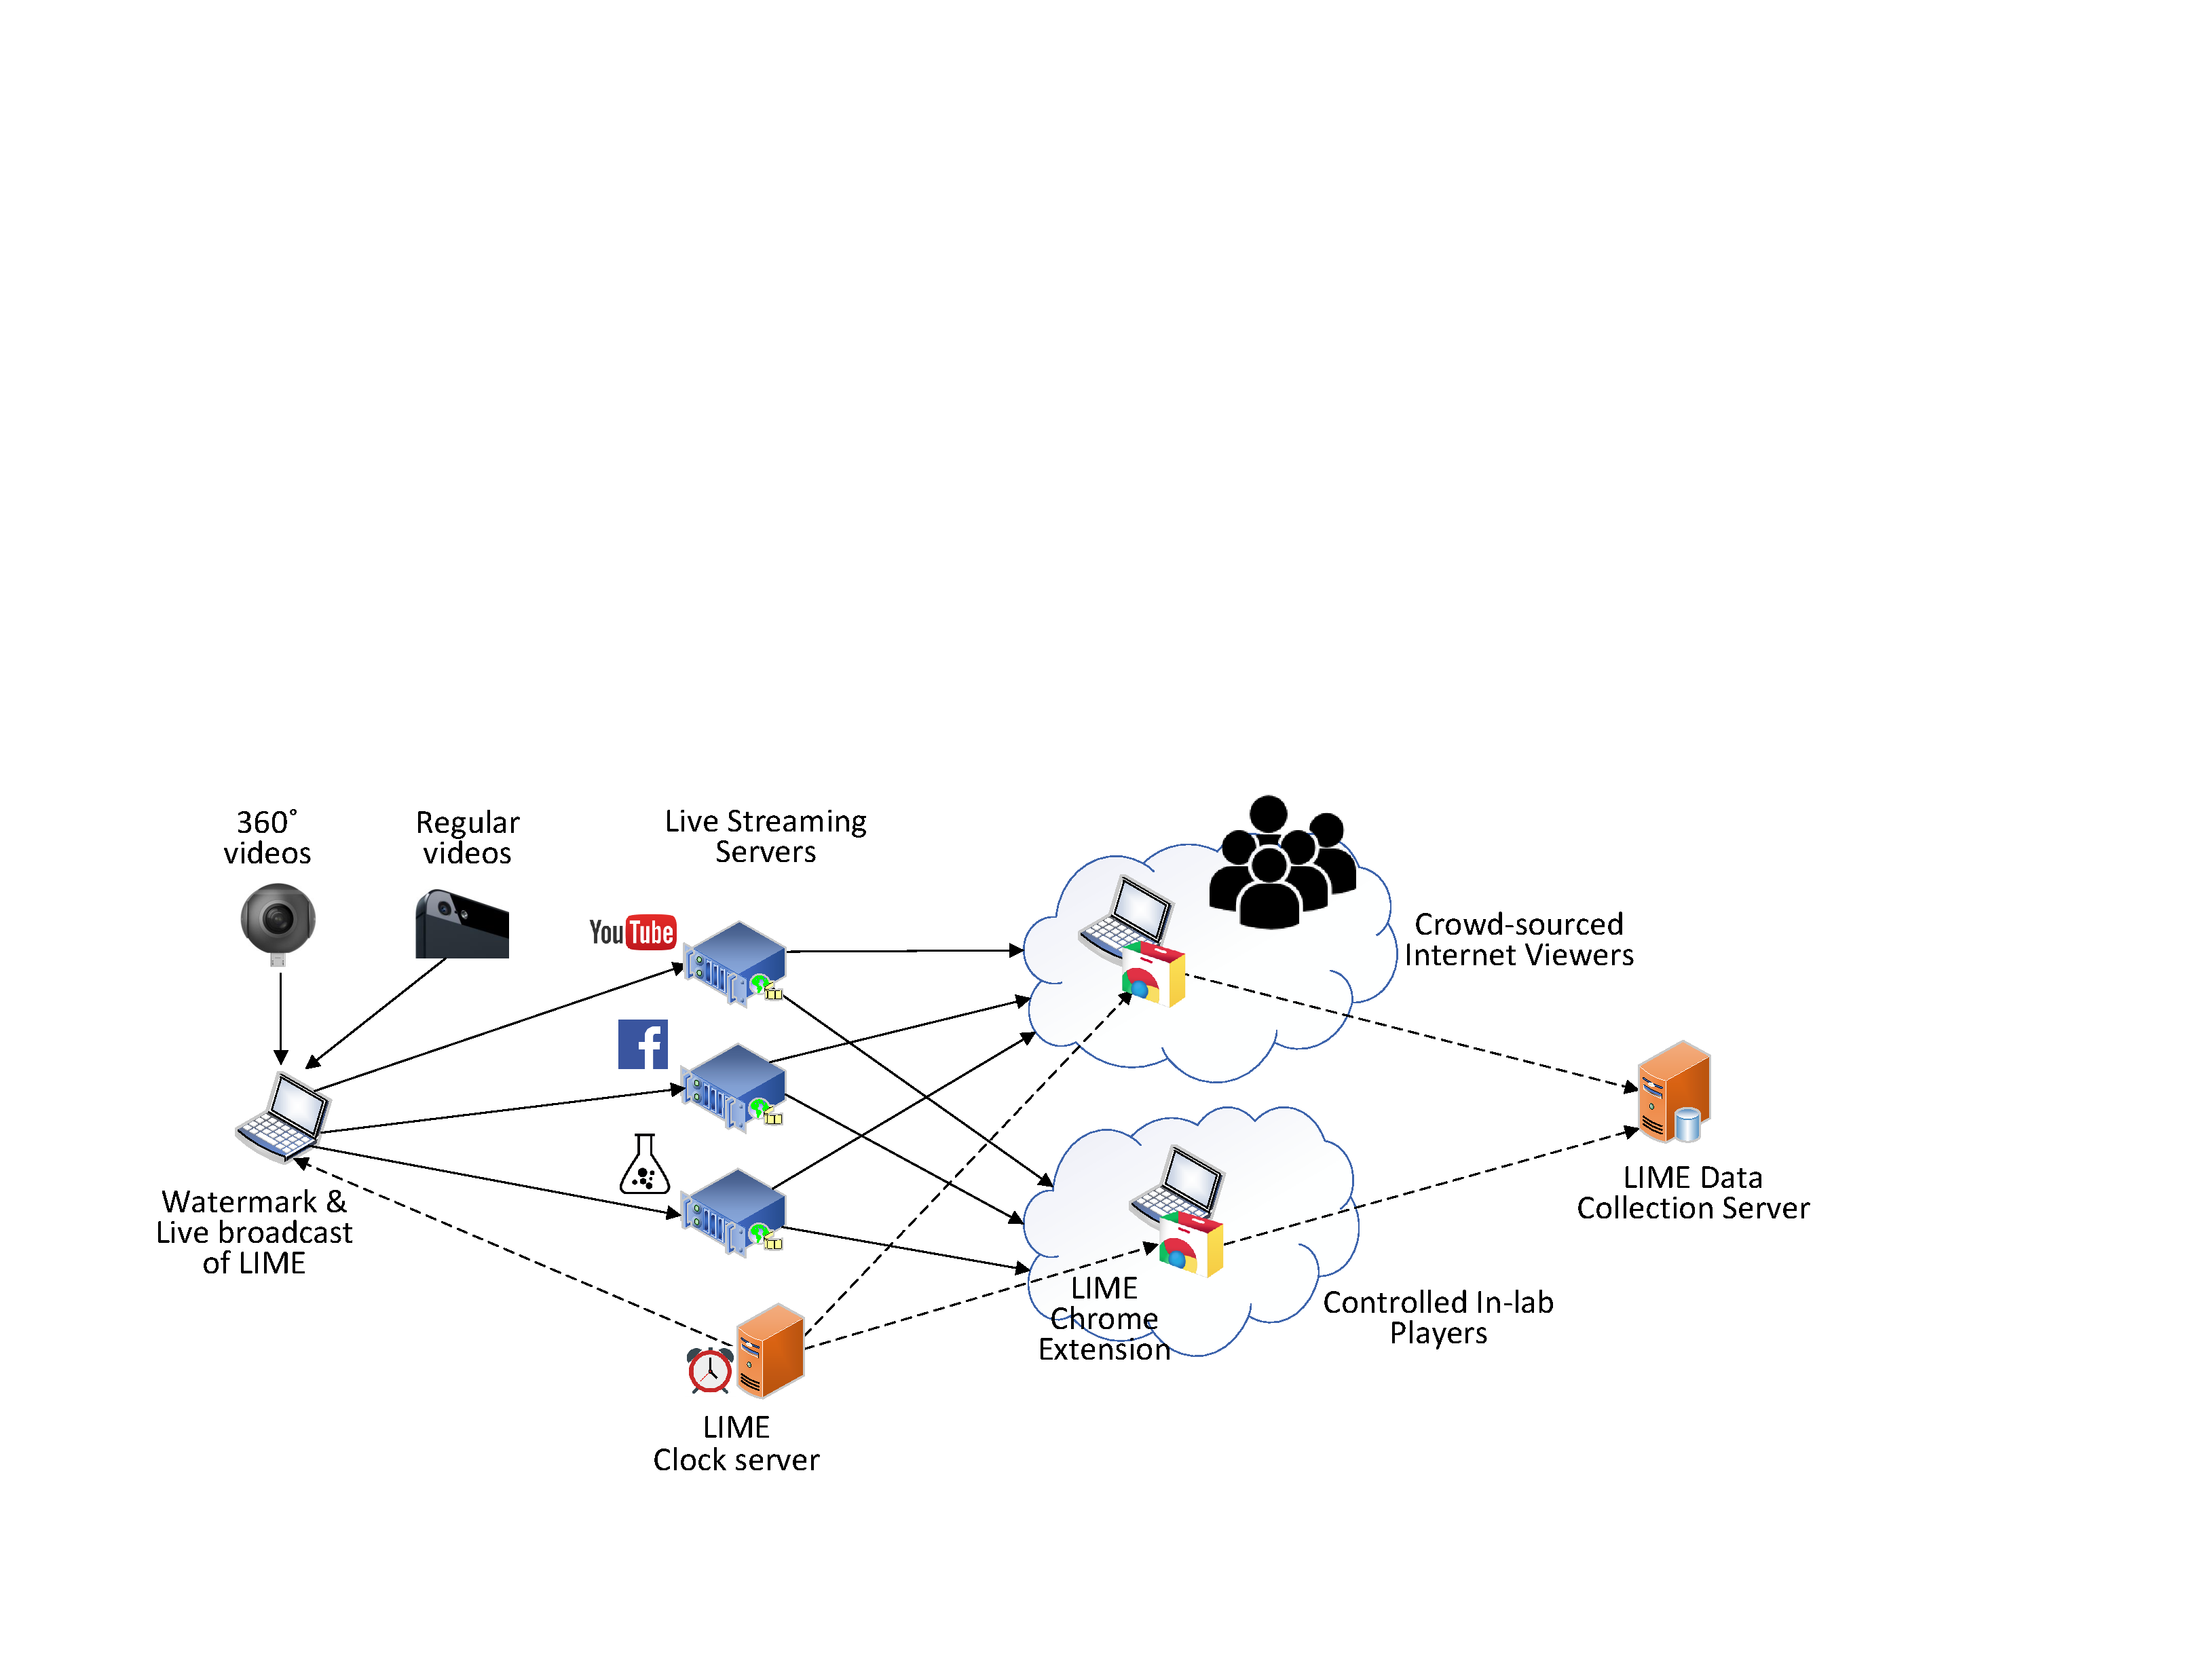
\includegraphics[width=0.9\textwidth]{figs/lime/testbed3.pdf}
	\end{center}
	%\vspace{-.2in}
	%\caption{System for collecting viewer-side performance statistics.}
	\caption{The system architecture of \lime.}
	%\vspace{-.2in}
	\label{fig:testbed}
\end{figure*}

%\mvnote{update figure accordingly}
Figure~\ref{fig:testbed} shows \lime's key components: the \emph{broadcaster}, \emph{streaming servers}, a set of \emph{viewers} (either crowd-sourced viewers or controlled players), the data collection server, and the clock server.
%
The broadcaster is a Linux machine instrumented with Open Broadcaster Software (OBS) Studio~\cite{obs} to broadcast pre-recorded videos to the target streaming servers, either commercial or controlled by the ``experimenter'' \emph{i.e.}, a researcher using \lime for her own studies. Such a ``replay'' approach ensures repeatable experiments.
%
The vast majority, if not all, of popular live streaming services (\eg YouTube, Facebook, Periscope, and Twitch) currently support OBS and can be thus tested via \lime.
%
The experimenter can use either a regular camera to shoot non-360\degree{} videos,
or a panoramic camera (\eg Insta360~\cite{insta360}) to capture 360\degree{} videos.
%
The viewers consist of both \emph{crowd-sourced} Internet viewers and \emph{in-lab} players.  To allow recruiting viewers in a short period of time, we integrate \lime with Amazon Mechanical Turk~\cite{mturk}, a popular crowd-sourcing platform.
%
The experimenter can thus select a number of target viewers (with specific locations/demographics if needed), how many videos they should watch, and their compensation. In-lab players consist of Chrome's instances equipped with \lime's Chrome extension (described next) which are automated via Selenium.\footnote{https://www.seleniumhq.org/}
%\mvnote{I know right know these instances are manually run, but I don't see an issue to integrate with selenium.}

\lime collects viewing statistics using a Google Chrome extension.
%We choose a browser extension because it is agnostic of the live streaming service, \eg commercial or not.
%
We choose a browser extension because it is lightweight, secure, and easy to install.
%agnostic of the live streaming service, \eg commercial or not.
%
Running in the background on the viewer side, the extension collects the following data summarized in Table~\ref{tab:datacollected}: (1) the video playback quality (\eg 720p), (2) stall (\ie rebuffering) events, (3) HTTP request/response headers, (4) user interactions such as dragging the mouse to change the viewport, and (5) periodically captured (every 2 seconds) screenshots of the visible portion of the video.

\begin{table}[]
	\centering
	\small
	\begin{tabular}{l|l|l}
		\multicolumn{1}{c|}{Item}  & \multicolumn{1}{c|}{API/Obj} & \multicolumn{1}{c}{Interval} \\
		\hline
		Video Quality Change & \texttt{HTML Player}     & Event Triggered \\
		Rebuffering Events   & \texttt{HTML Player}     & Event Triggered       \\
		HTTP Req/Res Headers & \texttt{chrome.debugger} & Event Triggered       \\
		User Interactions    & \texttt{HTML Window}     & Event Triggered       \\
		Video Screenshots    & \texttt{chrome.tabs}     & Every 2 Seconds    \\
	\end{tabular}
	\caption{Data items collected by \lime.}
	\label{tab:datacollected}
\end{table}

Finally, Figure~\ref{fig:testbed} shows that \lime further includes two servers under the experimenter's control: a \emph{data collection server} and a \emph{clock server}. The data collection server is the end-point where users' viewing statistics collected by the Chrome extension are uploaded to. The clock server provides synchronized clock readings to both the broadcaster and the viewers, in order to enable accurate measurement of the broadcaster-to-viewer latency. More details will be provided in~\S\ref{sec:b2v}.


\subsection{Measuring the Broadcaster-to-Viewer (B2V) Latency}
\label{sec:b2v_overview}
B2V latency is an important QoE metric for live streaming. We define it as the latency from when a frame leaves the broadcaster to when the frame is consumed by a viewer. A long B2V latency causes lags that are undesirable for real-time live events such as sports. One possible methodology of measuring B2V latency is as follows.
%
The broadcaster watermarks every frame $f$ with a timestamp $t_B(f)$
denoting the time when the frame is generated.
%to leverage timestamps watermarked at the broadcaster, denoted as $t_B$.
When the same frame $f$ is being played, the viewer obtains the current timestamp $t_V(f)$ from the clock server (Figure~\ref{fig:testbed}). Meanwhile, $t_B(f)$ can be extracted from the frame (we use Tesseract OCR~\cite{tesseract-ocr} to perform text recognition on screenshots).
The B2V latency for $f$ is therefore $t_V(f)-t_B(f)$.
%
Note that $t_B(f)$ is obtained from the same clock server as $t_V(f)$.
%
Also note that the originally obtained $t_B(f)$ and $t_V(f)$ need to be calibrated by subtracting the one-way latency to the clock server (estimated as half of the measured RTT).
%

The above scheme works for non-360\degree{} live videos. However,
we face two practical challenges when applying it to 360\degree{} live videos.
The first challenge relates to \emph{projection} used in 360\degree{} videos.
The OBS software can apply the watermark to only \emph{unprojected}
raw frames that contain the panoramic 360\degree{} views. During a playback,
a viewer's browser will apply the corresponding projection algorithm to display the visible portion. After projection, the timestamp watermark may be distorted, making OCR difficult.
%
To address this, we embed the watermark at a special spot (latitude = 0\degree{} and longitude = 0\degree{}) to minimize the distortion for equirectangular projection. Similar spots can be identified for other projection schemes.

The second challenge is that the Chrome Extension API allows our data collector to capture only the \emph{visible} portion of a panoramic frame that may not contain the watermark. A possible solution is to embed multiple watermarks that cover all possible viewing areas, but doing so will affect viewers' viewing experiences and make OCR challenging again due to distortions incurred by projection.
%
Instead, we introduce a \emph{helper player} that always ``looks'' at a fixed direction (\ie latitude = 0\degree{} and longitude = 0\degree{}) whose FoV contains the watermark.
%
During a live broadcast session, the helper player
continuously extracts $t_B(f)$ from the received frames
and sends $t_B(f)$ to the data collection server.
%
Note that for each frame, its $t_B(f)$ only needs to be extracted once
regardless of the number of viewers, so we need only one helper player per broadcaster.
%
When an actual viewer receives $f$, it does not need to perform watermark extraction; it
only needs to record its own $t_V(f)$ and send it to the data collection server, which can now compute the B2V latency for frame $f$ watched by this \emph{particular} viewer as $t_V(f) - t_B(f)$. Note that for both the helper player and actual viewers, their
communication with the data collection server can be performed offline if we do not need to know the B2V latency in real time. In this case, the helper player or a viewer will upload all frames' $t_B(f)$ ($t_V(f)$) values to the data collection server in a single batch.


\section{Data Collection Using LIME}
\label{sec:lime_data_collection}

We now detail the data collection procedure. Using a panoramic camera (Insta360~\cite{insta360}) attached to a smartphone, we shoot three 10-minute long 360\degree{} videos: (1) a city street view shot by mounting the camera on a car, (2) an on-campus walk shot by hand-holding the camera, and (3) a bicycle racing game shot with a stationarily placed camera. In the following, we refer to them as \emph{Street}, \emph{Campus}, and \emph{Racing}, respectively.

We use \lime's broadcaster to stream, overall, the three videos (\emph{Street}, \emph{Campus}, and \emph{Racing}) per platform (YT and FB), for a total of 6 live feeds.
%
We invite Internet users to participate in our IRB-approved study by installing \lime's Chrome extension and watching live videos.
%approved by IU IRB\# 1803800200 and AT\&T IRB\# 2018-170
Viewers can watch multiple live videos, but they are restricted to one video at a time and each video at most once. During the live video streaming, a viewer can freely change the viewport by interacting with the player (\eg dragging the mouse or swiping on the touchscreen).
%\mvnote{unless they use a laptop with a tactile screen, the latter cannot happen. We should find a place where to discuss this}.
We ask the viewer not to change the default \emph{auto} quality option in the player so that we can study YouTube and Facebook's built-in rate adaptation mechanism. Viewers are also required to watch a video for at least 4 minutes, after which they can end their task. Only at this time, the extension uploads the collected data to our server, without impacting the live video streaming experience.


\begin{figure}[t]
	\centering
	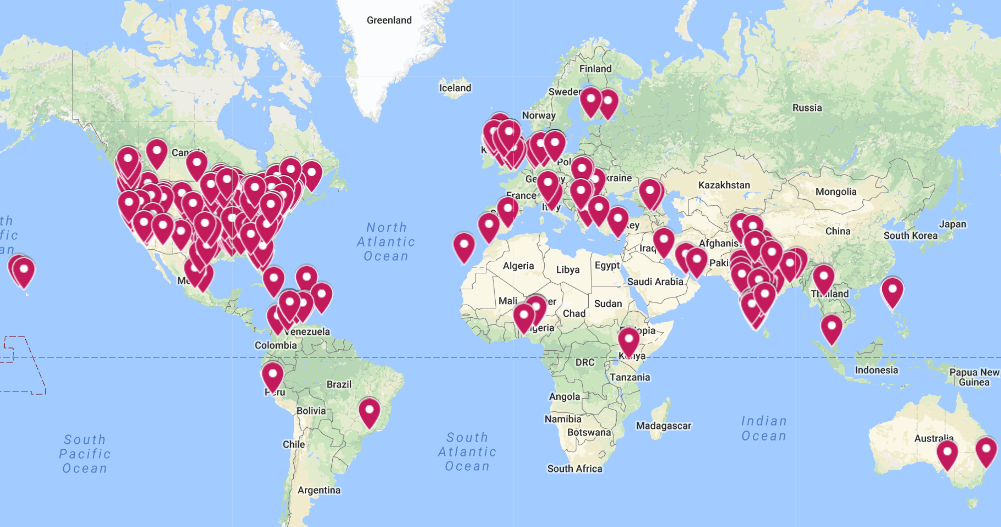
\includegraphics[width=.5\textwidth]{figs/lime/map4.png}
	\caption{Geographical distribution of paid AMT users.}
	\label{fig:map}
\end{figure}


During a 7-day study in May 2018, we kept our (replayed) live video feeds alive, and used Amazon Mechanical Turk (AMT) to recruit 548 paid viewers from 35 countries, with USA and India contributing 78\% of the viewers, as shown in Figure~\ref{fig:map}. Overall, we collected 22 GB data corresponding to more than 4,000 minutes of video viewing. Many paid viewers watched our feeds for more than 4 minutes.  To prevent bias toward viewers with long viewing time, our analysis focuses on only the first 4 minutes per viewer.
During the study, no personally identifiable information was collected.


\section{Understanding Commercial 360\degree{} Live Video Streaming in the Wild}
We now characterize the data collected in \S\ref{sec:lime_data_collection} to reveal the landscape of the performance of today’s popular live 360° video
streaming services.

\subsection{Basic viewer-side QoE metrics}
It is known that three key factors affect the QoE of regular video streaming (both live and on-demand): video quality, stall duration, and quality changes~\cite{yin2015control,huang2015buffer,mao2017neural,dimopoulos2015identifying}. These metrics are also important to panoramic live video streaming so we quantitatively measure them using the AMT dataset. We find that our three videos yield very similar distributions on all metrics. Thus, we present their aggregated results henceforth.

\begin{figure*}[t]
	\centering
	\begin{minipage}{.4\textwidth}
		\centering
		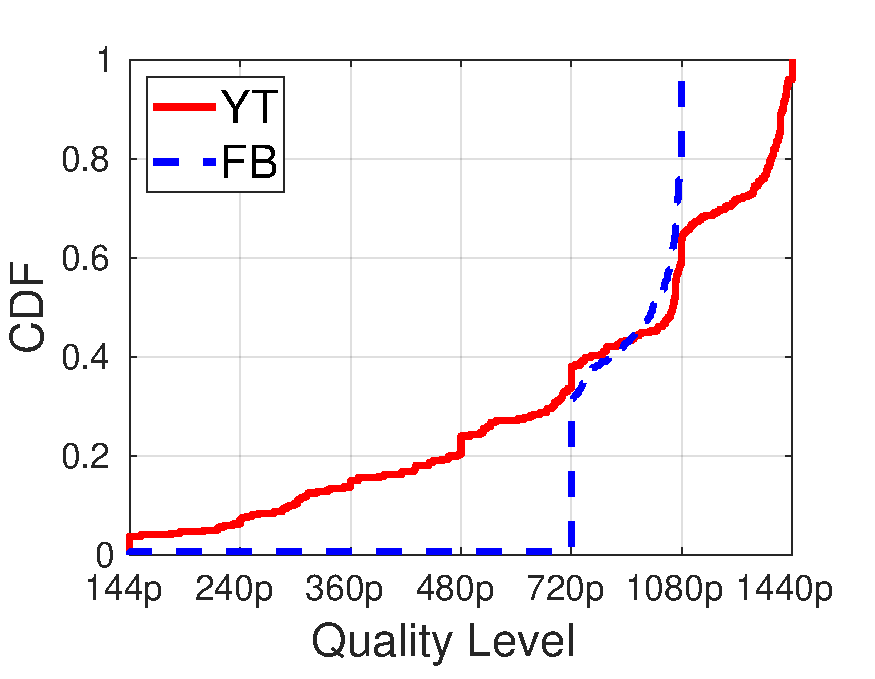
\includegraphics[width=\linewidth]{figs/lime/average_quality.pdf} \vspace{-.25in}
		\caption{\small Average streaming quality across all sessions.}
		\label{fig:average_quality}
	\end{minipage}
	\begin{minipage}{.4\textwidth}
		\centering
		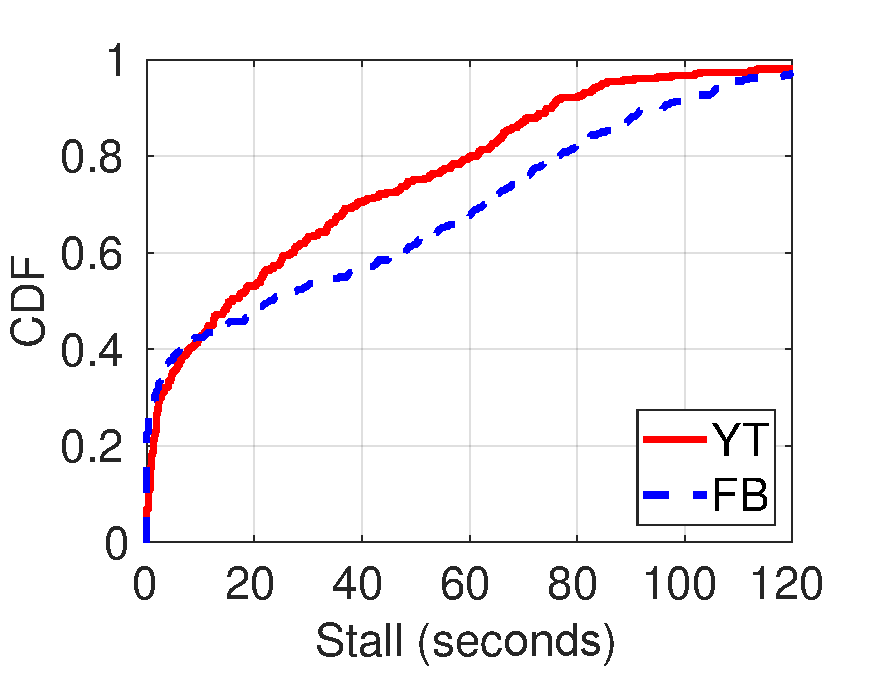
\includegraphics[width=\linewidth]{figs/lime/len_of_stall.pdf} \vspace{-.25in}
		\caption{\small Distributions of per-session stall duration.}
		\label{fig:stall_per_session}
	\end{minipage}
\end{figure*}


\BULLET \textbf{Video Quality.}
Figure~\ref{fig:average_quality} plots the Cumulative Distribution Function (CDF) of the average video quality for YT and FB across all viewing sessions. Recall that each viewing session is a 4-minute 360\degree{} live video content streamed to one paid AMT viewer. As shown in this figure, a key difference between YT and FB is that the average quality for most FB viewers is either 720p or 1080p, which are the only two quality levels provided by FB; in contrast, YT supports 7 quality levels ranging from 144p to 1440p, providing more flexibility as we will discuss shortly.
%a wide range of
%Despite this difference, the median video quality is similar: 4.9 for YT and 4.8 for FB (we use the following quality mapping throughout this paper: 0=144p, 1=240p, 2=360p, 3=480p, 4=720p, 5=1080p, 6=1440p).
Overall, the live 360\degree{} videos' quality is not high, with 34\% (35\%) of YT (FB) sessions having an average quality no higher than 720p.
%
It is important to note that the above qualities refer to the qualities of panoramic frames. Since a viewer perceives only a small portion of the panoramic scene (about 15\% as measured), the actual \emph{perceived} quality is much lower, \eg 15\% of the 720p resolution is between 240p and 360p.

\BULLET \textbf{Stall.} Figure~\ref{fig:stall_per_session} plots the CDFs of the stall duration per session. About 36\% (39\%) of YT (FB) sessions experience less than 5 seconds stalls. However, many users experience very long stalls: 47\% (52\%) of YT (FB) sessions stall for at least 20 seconds (\ie 5 seconds per minute). FB is afflicted by longer stalls than YT, despite their viewing  sessions characterized by similar throughput distributions. Given this, we are leaning towards attributing YT's shorter stall duration to its wider range of quality levels, which allow YT players to flexibly select (lower) streaming bitrates.

We also investigate how stalls are distributed within a session. We find that the vast majority of stall events, which are separated using an inter-stall time of at least 1 second, are fairly short: for YT (FB), the median of their durations are 0.7 (1.0) second.  Note that changing the threshold of inter-stall time to 0.5s or 1.5s yields similar results. 
%
Meanwhile, the number of stall events is large. Figure~\ref{fig:stall_num} plots the CDFs of the number of stall events per session, with the median measured to be 18 (17) for YT (FB), respectively. Compared to fewer long stall events, having more short stall events may bring even worse QoE (\eg motion sickness in VR)~\cite{duanmu2017qoe, moorthy2012qoe, qi06qoe}. %in particular in the VR context. \feng{[[Any paper to cite?]]}

\begin{figure*}[t]
	\centering
	\begin{minipage}{.4\textwidth}
		\centering
		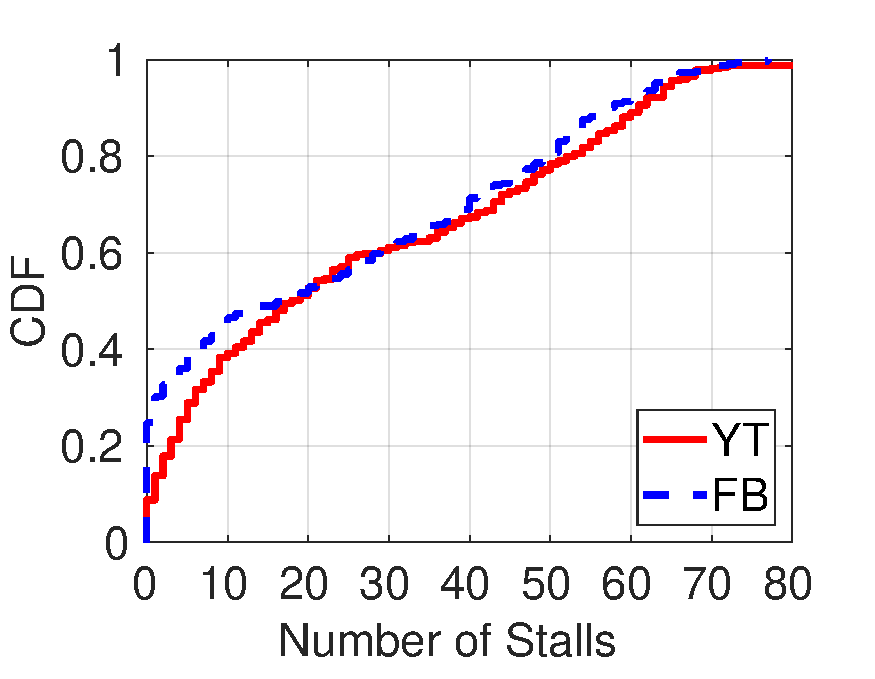
\includegraphics[width=\linewidth]{figs/lime/num_of_stalls.pdf} \vspace{-.25in}
		\caption{\small Distributions of per-session number of stalls.}
		\label{fig:stall_num}
	\end{minipage}
	\begin{minipage}{.4\textwidth}
		\centering
		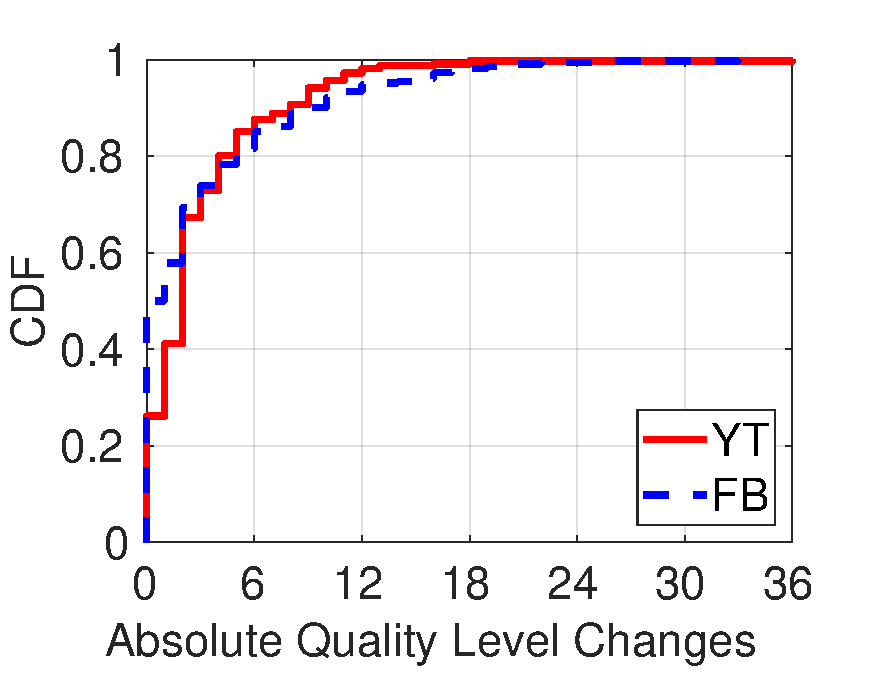
\includegraphics[width=\linewidth]{figs/lime/quality_change.pdf} \vspace{-.25in}
		\caption{\small Distributions of per-session quality level changes.}
		\label{fig:quality_change}
	\end{minipage}
\end{figure*}


%\mvnote{All this need more attention on the bottleneck introduced by the client as discussed.}
Since the stall duration shown in Figure~\ref{fig:stall_per_session} appears to be much higher than those measured by a previous study on Periscope~\cite{siekkinen16}, we attempt to find out the reason. Recall that live video streaming consists of four phases: upload, server-side re-encoding, download, and client-side rendering/playback.
For upload, we ensure high bandwidth between our broadcaster and the streaming servers.
For download, surprisingly, we observe very little correlation between
the per-session stall duration and its network throughput or throughput variation
(Pearson correlation coefficient $<$ 0.1). In fact, many viewers have very high network throughput but still experience high stalls (recall that YouTube can reduce its quality to as low as 144p). For example, one-third of the top 30\% YT sessions in terms of the stall duration are characterized by an average throughput ranked in the top 30\% of the sessions.
%For example, for the top 30\% YT sessions experiencing highest stall durations, 32\% have their average HTTP response throughput ranked at top 30\%.

The above observation makes us believe that for live 360\degree{} video streaming, the performance bottleneck is caused by either the server processing (real-time video re-encoding and possibly projection transformation) or client-side computation/rendering.
%
In particular, we are able to verify that the \emph{client-side overhead} can cause frequent stalls:
when testing on a 2013 MacBook Pro, we observe the CPU utilization of 360\degree{} live streaming can reach up to 80\%, about 60\% higher than non-360\degree{} live streaming. When the CPU is saturated, the live streaming can oftentimes stall.

%which needs to perform real-time video re-encoding and (possibly for 360\DEG videos) projection transformation, which incur high overheads.

\BULLET \textbf{Quality Changes.} Figure~\ref{fig:quality_change} plots the CDFs of the total number of quality level changes per session. When a quality level change occurs, it is counted as $\Delta L = |L_\text{before} - L_\text{after}|$ where $L_\text{before}$ and $L_\text{after}$ are the quality levels before and after the change, respectively. Possible levels are \{0,1,...,6\} for YT and \{4,5\} for FB\footnote{We use the following quality mappings throughout this paper: 0=144p, 1=240p, 2=360p, 3=480p, 4=720p, 5=1080p, 6=1440p.}. We then sum up all $\Delta L$ to get the total quality level changes per session.
%
For most sessions, we did not observe significant quality changes: the median of $\sum\Delta L$ is only 2 and 1 for YT and FB, respectively.
%This is likely attributed to conservative rate adaptation schemes for live streaming that under-utilize the available bandwidth (see \S\ref{sec:xx}).
Nevertheless, we do find about 6\% (10\%) for YT (FB) of sessions with $\sum\Delta L \ge 10$, attributed to the highly variable bandwidth as confirmed from our measured network throughput.



\subsection{Broadcaster-to-viewer (B2V) Latency}
\label{sec:b2v}

\begin{figure}[t]
	\centering
	\centering
	\small
	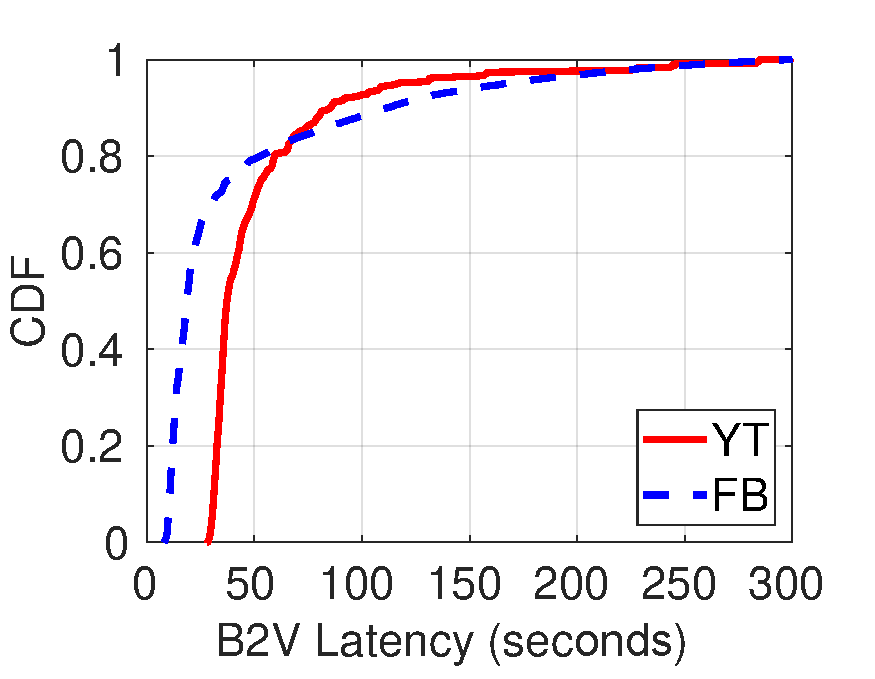
\includegraphics[width=0.4\textwidth]{figs/lime/e2e_latency.pdf}
	\caption{B2V latency of samples across all sessions. In each session, B2V latency is measured every 2 seconds.}
	\label{fig:e2e_latency}
\end{figure}

We apply the method introduced in~\S\ref{sec:b2v_overview} to measure the B2V latency for the AMT viewers, with the results shown in Figure~\ref{fig:e2e_latency}. %We show the results in Figure~\ref{fig:e2e_latency}.
%
We make three observations.
%
First, most sessions have consistent B2V latencies, around 18.7 seconds for FB and 37.1 seconds for YT (median values). Overall, the observed B2V latency is much higher compared to previous measurement on Periscope~\cite{wang16}, which uses push-based RTMP on a subset of users to provide an ultra-low B2V latency (less than 2 seconds).
%\feng{[[Xing: a quick experiment to compare B2V latency between 360 and non-360 live?]]}
%
Second, both platforms exhibit long tails of up to 4.8 minutes for FB and 5.1 minutes for YT. Such high latency inevitably affects viewers' experience.
Although it is difficult to reverse engineer the precise algorithm, we find that throughput appears to be a factor that affects the B2V latency. For example, YT exhibits a negative correlation (Pearson correlation coefficient of -0.4) between the B2V latency and throughput.
%
Third, we also notice that FB exhibits lower B2V latency than YT.
%This can be partly explained by several
This can be explained by several potential reasons.
%
One is that compared to YT, FB has a shorter chunk duration (1 vs 5 seconds) that leads to a lower chunking delay~\cite{wang16}. FB also has a lower polling delay allowing the viewer to update the chunk list more quickly. In addition, recall that a FB server only re-encodes the input video into 2 quality levels while a YT server needs to process 7 quality levels up to 1440p. Such a higher re-encoding overhead may also contribute additional latency.


\section{Adaptiveness in 360\degree{} Live Video Streaming}

We complement our crowd-sourced study with controlled
experiments to shed light on bringing adaptiveness to both
the viewers and the broadcaster. These are the key features
missing from today’s 360\degree{} live video streaming systems. The contribution here
is to quantitatively study its benefits using commercial systems,
realistic live 360\degree{} video content, and real users’ viewing trajectory
traces. In addition, we also identify several inefficiencies in production
360\degree{} live video streaming systems that diminish the benefits of
viewport adaptiveness. We conduct all controlled experiments over
\lime by replacing crowd-sourced viewers with in-lab players. The preliminary results will be discussed in the proposal presentation.
